In satellite \gls{qkd}, the quantum information is synchronized by transmitting along with the classical one. Figure~\ref{fig:qkd_satellite} shows a high-level view of this schematic.

\begin{figure}[htbp]
    \centering
    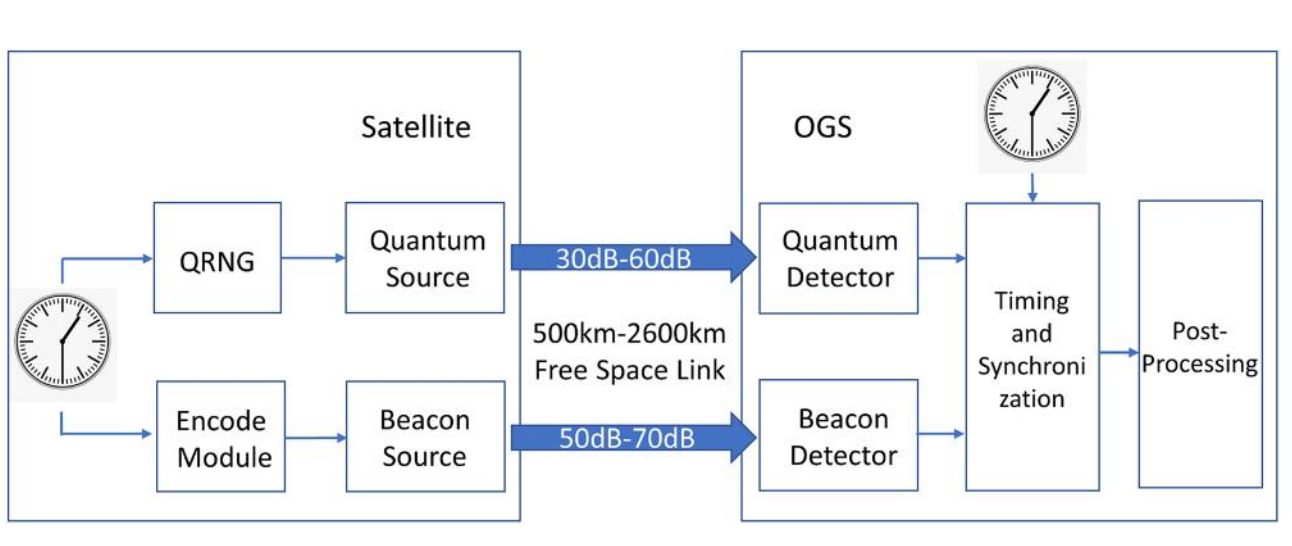
\includegraphics[scale=0.3]{fig/SatelliterQKD.png}
    \caption{High-level satellite Quantum Key Distribution timing and synchronization schematic \cite{zhang2021timing}.}
    \label{fig:qkd_satellite}
\end{figure}

At the beacon source, a de Bruijn sequence is modulated before transmitting to the ground.

The encode process happens at the satellite, where it uses the \gls{lfsr} algorithm to generate a positioning sequence (of order $k$ for example). The prerequisite of finding a proper primitive polynomial is the main drawback of this encoder. 

The decoding process takes place at the ground station, a look-up table is used to identify the unique position of the received sequences of length $k$. The complexity of this method is exponential.

Furthermore, in this model, a sequence of beacon pulses is used to represent a binary de Bruijn sequence. Considering the timing jitter performance, a long period of no-pulses should be forbidden. If one pulse slot is used to represent a binary bit, for example, on is 1 and off is 0, a long run of 0's in the sequence (which is a long period of no-pulses) would impact the timing jitter. In \cite{zhang2021timing}, two pulse slots are used to represent a single bit (on-on is 1 and on-off is 0) so that one can avoid two consecutive no-pulses. The transmitted sequence is called \gls{HdB}. However, the above scheme requires $2n$ pulse slots to represent a de Bruijn sequence of length $n$ and needs to receive a sub-sequence of $2 \log n$ pulse slots to locate its position. Formally, the \gls{HdB} sequence's rate is just $0.5$, where rate is a quantity that needs to be as high as possible (the definition of sequences' rate is given in section \ref{sec:rate}).

% For further illustration, the whole process, methods, and drawbacks of \gls{dBTS} system using \gls{HdB} sequence is summarized is figure \ref{fig:dBTS}
% \begin{figure}[htbp]
%     \centering
%     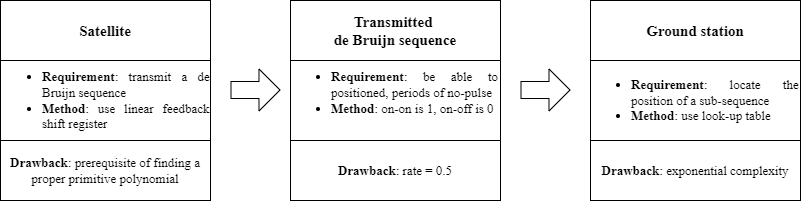
\includegraphics[scale=0.5]{fig/dBTS.png}
%     \caption{de Bruijn based timing and synchronizing system use Hybrid de Bruijn code}
%     \label{fig:dBTS}
% \end{figure}

Table \ref{tab:dBTS} summarized the process, applied methods and drawbacks of \gls{dBTS} system using \gls{HdB} sequence.
\begin{table}[htbp]
    \centering
    \caption{Timing and synchronizing system use Hybrid de Bruijn code.}
    \renewcommand{\arraystretch}{1.25}
    \resizebox{\columnwidth}{!}{
    \begin{tabular}{| p{4.1cm} | p{4.1cm}| p{4.1cm} |}
    % \begin{tabular}{|l|l|l|}
        \hline
        \textbf{Satellite} & \textbf{Transmited de Bruijn sequence} & \textbf{Ground Station} \\
        \hline \hline
        \textbf{Requirement}: transmit a de Bruijn sequence of order $k$
          &
        \textbf{Requirement}: be able to be positioned, avoid periods of no-pulse 
          &
        \textbf{Requirement}: locate the position of any length $k$ subsequence  \\
        \hline
        \textbf{Method}: use linear feedback shift register algorithm
          &
        \textbf{Method}: modulate on-on is $1$, on-off is $0$
          &
        \textbf{Method}: use look-up table \\
         \hline 
        \textbf{Drawback}: the prerequisite of finding a proper primitive polynomial 
        &
        \textbf{Drawback}: rate is $0.5$
        &
        \textbf{Drawback}: exponential complexity \\
        \hline
    \end{tabular}
    }
    \label{tab:dBTS}
    
\end{table}

This thesis's target is to surmount the drawbacks listed above.

% The main task here is designing a code satisfying the constraints of \gls{dBTS} system.

% \textbf{Problem Statement}: Designing a high rate sequence which is capable of positioning and avoids two consecutive symbol $0$'s.

In order to avoid long period of no pulse, the positioning sequences are combined with run length limited constraints. Such sequences are called Run length limited de Bruijn (RdB) sequences, presented in chapter \ref{chapter:RdB}. The \gls{RdB} sequences are not just suitable with \gls{dBTS} system, but also have a higher rate than \gls{HdB} sequences. More precisely, rate of the longest \gls{RdB} sequences are \[\log\left(\dfrac{1+\sqrt{5}}{2}\right)\approx0.6942.\]

So as to generate one of the longest \gls{RdB} sequences, based on \gls{fkm} algorithm, chapter~\ref{chapter:pro_rlldb_sequence} provides an encoder whose time complexity is constant amortized time per symbol. Moreover, to locate the position of an arbitrary proper subsequence in the whole \gls{RdB} sequence, a decoder is also presented. The proposed decoder modifies the decoding algorithm found by \citeauthor{kociumaka2016efficient} in~\cite{kociumaka2016efficient}, which is currently the state of the art method to position a subsequence in the de Bruijn sequence, and therefore, is better than look-up table.

Beside, the \gls{RdB} sequence is even more general and adaptive. More particularly, when the constraint of forbidding pattern $00$ is relaxed, that is, a longer run of bit $0$'s is allowed, the \gls{RdB} sequence can be easily adjusted to make the its rate higher and still suits the system. 